\documentclass{article}
\usepackage{NIPS10,times}
%\documentstyle[nips07submit_09,times]{article}
\usepackage[square,numbers]{natbib}
\usepackage{amsmath, epsfig}
\usepackage{amsfonts}
\usepackage{subfigure}
\usepackage{graphicx}
\usepackage{amsfonts}
\usepackage{algorithm}
\usepackage{algorithmic}
\usepackage{easybmat}
\usepackage{listings}
\usepackage{footmisc}
\renewcommand\algorithmiccomment[1]{// \textit{#1}}
%
\newcommand{\ignore}[1]{}
\newcommand{\comment}[1]{}
\DeclareMathOperator*{\argmax}{arg\,max}

% decrease spacing in itemize
\newenvironment{itemize*}{
\begin{itemize}
  \setlength{\itemsep}{0.7em}
  \setlength{\parskip}{0pt}
  \setlength{\parsep}{0pt}
}{\end{itemize}}

\title{Introduction to Data Science\\Homework Assignment 3}

\author{
Michael Discenza\\\\
Columbia University, New York, NY 10027, USA \\
\texttt{mad2200@columbia.edu}
}
}

% The \author macro works with any number of authors. There are two commands
% used to separate the names and addresses of multiple authors: \And and \AND.
%
% Using \And between authors leaves it to \LaTeX{} to determine where to break
% the lines. Using \AND forces a linebreak at that point. So, if \LaTeX{}
% puts 3 of 4 authors names on the first line, and the last on the second
% line, try using \AND instead of \And before the third author name.

\newcommand{\fix}{\marginpar{FIX}}
\newcommand{\new}{\marginpar{NEW}}
\newcommand{\X}{\mathcal{X}}

\nipsfinalcopy

\begin{document}

\maketitle



%%%%%%%%%%%%%%%%%%%%%%%%%%%%%%%%%%%%%%%%%%%%%%%%%%%%%%%%%%%%%%%%%%%%%%%%%%%%%%%%%%%%%%%%%%
%%%%%%%%%%%%%%%%%%%%%%%%%%%%%%%%%%%%%%%%%%%%%%%%%%%%%%%%%%%%%%%%%%%%%%%%%%%%%%%%%%%%%%%%%%
%%%%%%%%%%%%%%%%%%%%%%%%%%%%%%%%%%%%%%%%%%%%%%%%%%%%%%%%%%%%%%%%%%%%%%%%%%%%%%%%%%%%%%%%%%

\section{FlowingData.com Visualization Tutorial}

I tried to recreate 


% latex table generated in R 2.15.1 by xtable 1.7-0 package
% Mon Oct 22 22:36:55 2012
\begin{table}[ht]
\begin{center}
\begin{tabular}{rlrrrrrr}
  \hline
 & Occupational Group & Number of Women & Women's Earnings & Number of Men & Men's earnings & Percentage Women\_women & Total Size\\ 
  \hline
1 &   Management occupations & 4535000 & 979 & 6687000 & 1384 & 0.40 & 11222000 \\ 
  2 &   Business and financial operations occupations & 2928000 & 885 & 2159000 & 1167 & 0.58 & 5087000 \\ 
  3 &   Computer and mathematical occupations & 828000 & 1088 & 2516000 & 1320 & 0.25 & 3344000 \\ 
  4 &   Architecture and engineering occupations & 334000 & 1001 & 2319000 & 1286 & 0.13 & 2653000 \\ 
  5 &   Life, physical, and social science occupations & 477000 & 931 & 603000 & 1156 & 0.44 & 1080000 \\ 
  6 &   Community and social services occupations & 1117000 & 753 & 791000 & 860 & 0.59 & 1908000 \\ 
  7 &   Legal occupations & 693000 & 962 & 506000 & 1696 & 0.58 & 1199000 \\ 
  8 &   Education, training, and library occupations & 4883000 & 818 & 1794000 & 1020 & 0.73 & 6677000 \\ 
  9 &   Arts, design, entertainment, sports, and media occupations & 689000 & 777 & 882000 & 951 & 0.44 & 1571000 \\ 
  10 &  Healthcare practitioner and technical occupations & 4052000 & 909 & 1362000 & 1210 & 0.75 & 5414000 \\ 
   \hline
\end{tabular}
\end{center}
\end{table}

\begin{figure}[H]
\begin{center}
\includegraphics[width=1\columnwidth]{gender.eps}
\caption{}
\end{center}
\end{figure}

\begin{figure}[H]
\begin{center}
\includegraphics[width=1\columnwidth]{gender.eps}
\caption{}
\end{center}
\end{figure}

\section{The Data Science of Art}


\section{Finance; Time Series and Regression}
[Kaushik Reddy and I spent a few hours working together on the code and then split up for the remainder of the project due to schedule constraints]

\begin{figure}[H]
\begin{center}
\includegraphics[width=1\columnwidth]{IBM_log_return.eps}
\caption{}
\end{center}
\end{figure}


\begin{figure}[H]
\begin{center}
\includegraphics[width=1\columnwidth]{IBM_log_volume.eps}
\caption{}
\end{center}
\end{figure}


I fit a model by regressing log returns on the previous two days' returns (an autoregressive second order model).  This procedure was conducted by manually lagging the data and using the two previous days' log returns as perdictor vectors, not using the AR or ARIMA functions. I did fit an AR function that found the optimal number of predictors to be 36 using AIC as the selection criterion for the model, but was unable to use the model with R's predict function and such a model would likely have been tremendously overfit. 

In the second order autoregressive model, the log returns of the previous day proved to be significant.
% latex table generated in R 2.15.1 by xtable 1.7-0 package
% Mon Oct 22 09:45:38 2012
% latex table generated in R 2.15.1 by xtable 1.7-0 package
% Mon Oct 22 11:08:46 2012
\begin{table}[ht]
\begin{center}
\begin{tabular}{rrrrr}
  \hline
 & Estimate & Std. Error & t value & Pr($>$$|$t$|$) \\ 
  \hline
(Intercept) & 0.0001 & 0.0004 & 0.26 & 0.7919 \\ 
  Predictor1 & -0.0502 & 0.0190 & -2.64 & 0.0083 \\ 
  Predictor2 & -0.0149 & 0.0190 & -0.79 & 0.4318 \\ 
   \hline
\end{tabular}
\end{center}
\end{table} 
Despite the significance of the coefficients fit by the model, the signal was week and often times not in the right direction of the log return.  Run over the course of two years (on totally new test data after the model was fit to the previous 10 years of training data), the model earned a log return of -0.2447558, meaning that with this model, one would actually lose money.

This resulting log return is however based on a number of simplifying assumptions: 1) there are zero transaction fees, 2)when the model predicts either a positive or a negative return correctly, it makes the full log return associated with that day regardless of whether it was on the positive or negative side [i.e., the options market for purchasing shorts is perfectly efficient], 3) the model was not updated over time- it was only fit to the training data and was not recalibrated to either forget previous data points over time or incorporate new data as time progressed.

\begin{figure}[H]
\begin{center}
\includegraphics[width=1\columnwidth]{performance.eps}
\caption{This graph shows the performance of the model over the last 50 days of tranding.  When the red prediction line and the black line for actual log return have the same sign, the trading strategy makes money, and when they have opposite sides, it loses money}
\end{center}
\end{figure}


\begin{figure}[H]
\begin{center}
\includegraphics[width=1\columnwidth]{pl.eps}
\caption{An ideal cumulative P&L graph would show a steady growth in profits.  This model failed to produce a steady trajecotry or profitability}
\end{center}
\end{figure}


\section{Code Appendix}
All code (in easier to read form) as well as additional graphics files can be found on this assignment's git repository:
https://github.com/mdiscenza/HW3




%%%%%%%%%%%%%%%%%%%%%%%%%%%%%%%%%%%%%%%%%%%%%%%%%%%%%%%%%%%%%%%%%%%%%%%%%%%%%%%%%%%%%%%%%%
%%%%%%%%%%%%%%%%%%%%%%%%%%%%%%%%%%%%%%%%%%%%%%%%%%%%%%%%%%%%%%%%%%%%%%%%%%%%%%%%%%%%%%%%%%
%%%%%%%%%%%%%%%%%%%%%%%%%%%%%%%%%%%%%%%%%%%%%%%%%%%%%%%%%%%%%%%%%%%%%%%%%%%%%%%%%%%%%%%%%%



\begin{small}
\bibliographystyle{plainnat}
\bibliography{References} 
\end{small}
\end{document}
